\begin{document}
	
\newgeometry{left=2cm,right=2cm,bottom=1cm,top=1cm}
\pagestyle{empty}
\vfill
\vspace*{4cm}
\centerline{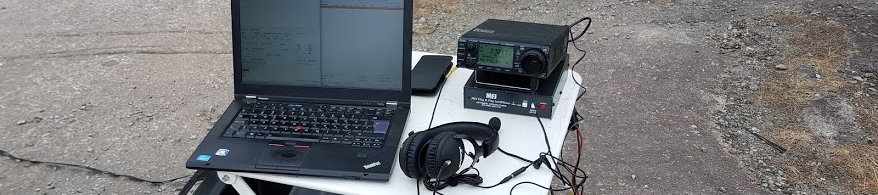
\includegraphics[width=\paperwidth]{logo/rubrikbild}}
\begin{flushright}
	\Huge{\bfseries{\TitleText}} \\[3mm]
	\Large{\bfseries{\SubtitleText}}
\end{flushright}

\vfill
	
Version: \DokVersion\ \hfill SMØUEI \hfill Datum: \DokumentDatum

\newpage

\newgeometry{top=3cm}

\pagestyle{fancy}
\lhead{\leftmark}
\rhead{
	\scriptsize
	\begin{tabular}{ll}
		\textbf{Version} & \textbf{Datum}\\
		\ \DokVersion & \DokumentDatum\\
	\end{tabular}
}

\chead{}

\lfoot{
	\scriptsize
	www.sm0uei.se
}

\cfoot{\scriptsize \thepage\ / \pageref{LastPage}}

\rfoot{\scriptsize
	anders@sikvall.se
}

\renewcommand{\footrulewidth}{0.2pt}

\widowpenalty=9999
\clubpenalty=9999

%	\setlength{\headsep}{1em}2

\cleardoublepage

%%% Innehållsförteckning
\tableofcontents

\newpage

\setlength{\parskip}{0.5em}
\setlength{\parindent}{0pt}

\section*{Förord}
	
Detta är den uppdaterade utgåvan för november 2023. Det var ett tag
sedan som jag ägnade mig åt det här alstret och det har kommit in lite
påpekanden om rättningar och att repeaterlistor med mera varit ganska
utdaterade. Det är förstås helt riktigt och jag har i skrivande stund
faktiskt försökt få in den färskaste informationen som finns från SSA.

Mycket har hänt sedan föregående information. Jag har flyttat från
Stockholm och har numera blivit SM5UEI men hänger fortfarande på
Kvarnbergets amatörradioklubb på torsdagskvällarna så där är det öppet
hus dessa dagar från kl. 19:00 när ni alla är välkomna att kika förbi.

Ändringar som skett sedan förra utgåvan:

\begin{itemize}[]
	\item Landsprefixdelen har kortats av och delats upp lite enligt 
	input från SMØMPV.
	\item Bandplanerna har setts över, bl.a. 60\,m-bandet i HF-delen 
	har lagts till då det saknades tidigare.
	\item Repeaterlistan uppdaterad med senaste data från SSA
	\item Gjort om några exempel-QSO enligt tips från SMØMPV
	\item En hel hoper med uppsnyggningar och förbättringar här och där.
\end{itemize}

Bidrag till handboken tas tacksamt mot men jag kommer bedöma ifall
materialet är lämpligt att ta med.  Hela materialet finns numera också
på Github om man vill gräva i det och fixa-dona, komma med 
förbättrings\-förslag och annat kul så finns den på följande länk:

\href{https://github.com/sikvall/rhb/}{https://github.com/sikvall/rhb}

Har ni en massa bra förslag på grejer som ni skulle vilja ha med i boken
så låt mig veta det där, det går också om ni vill arbeta in ändringar direkt
och skicka mig en s.k. "pull request" så kan jag kika på det. Det går också
att logga issues om man hittar fel.

Det går också hitta en massa annat radiorelaterat på min hemsida om ni 
är intresserade och där kan ni också normalt hitta radiohandboken som 
senaste version i PDF att ladda ner direkt.

\href{https://sikvall.se}{https://sikvall.se/}

Och kör radio där ute. Mobilt. Stabilt. Maritimt. Aeromobilt. Alltid med stil.\\[4em]

Karlholm, \DokumentDatum\\
\textit{Täpp-Anders Sikvall\\
	SM5UEI}

\clearpage

\section*{Nyheter i denna utgåva}

\subsection*{Instegscertifikat för amatörradio}

Den största nyheten sedan föregående version av radiohandboken är att PTS has nu tagit beslut om instegscertifikat för amatörradio och i denna version av radiohandboken finns det med en del ny information om detta som kan vara intressant för dig som funderar på att ta ett sådant certifikat. Detta har förlagts i en liten egen del i radiohandboken. Se mer i avsnitt \ref{sec:instegscertifikat} där detta beskrivs mer i detalj vad det innebär.

\subsection*{IEEE frekvensbandsbenämningar}

Frekvensbandsbeteckningar enligt IEEE har tillförts i sektion \ref{sec:IEEE-benamningar}.

\clearpage
	
